\mychapter{vision}{Vision, concepts and principles}
\begin{figure}
  \begin{center}
    \centerline{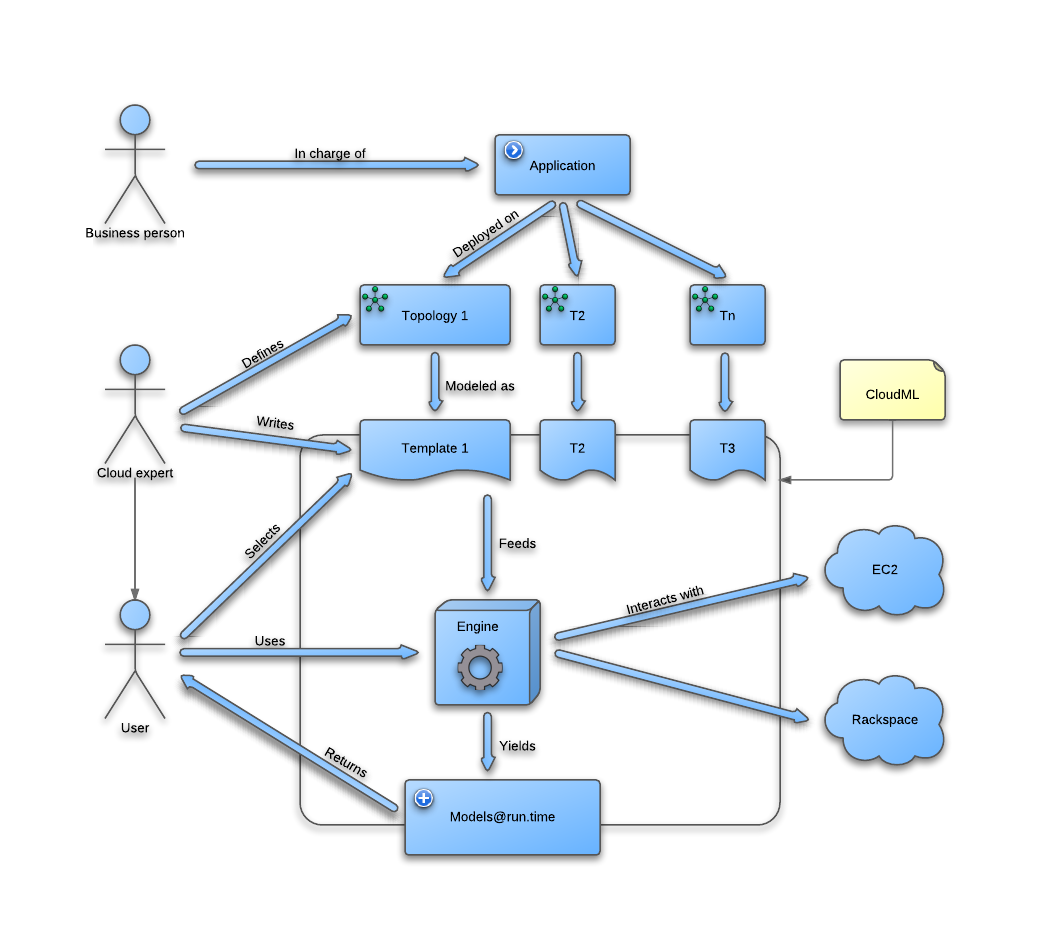
\includegraphics[width=1.5\linewidth]{img/big-picture.png}}
    \caption{``Big picture'', overview of CloudML procedure flow.}
    \label{fig:big-picture}
  \end{center}
\end{figure}


In this chapter the core approach and steps on the research to implementing CloudML will be described.
In the previous chapters, \citechap{challenges} and \citechap{requirements}, 
challenges and requirements were identified and described.
In this part of the thesis (\emph{contribution}) the challenges will be addressed 
by applying and implementing the requirements.

There are four main steps from start of the problem to an functional implementation.
\begin{enumerate}
  \item Identify and research in \emph{state of the art}.
  \item Recognize \emph{challenges}.
  \item Determine \emph{requirements} based on \emph{challenges}.
  \item \emph{Analyze} solutions, tools and procedure to implement \emph{requirements}.
  \item \emph{Implement} a solution based on \emph{analyzed} results.
\end{enumerate}
Of these steps step $1$ (one) to $3$ (three) are already covered by \citechap{state-of-the-art}
, \citechap{challenges} and \citechap{requirements}.
This chapter is an intermediate chapter which will introduce the chapter of \citechap{design}
and \citechap{implementation}.

\section{Core vision and concept}

\note{Note: This part of this section is almost direct copy/paste of what was already here,
might not seem to "fit in"}
\todo{Maybe remove, thoughts?}

The core envision is to solve requirements from~\citechap{requirements} by applying a 
model-driven approach supported by modern technologies.
The concept and principle of CloudML is to be an easier and more reliable
path into cloud computing for IT-driven businesses of variable sizes.
The tool is envisioned to parse and execute template files representing topologies
of instances in the cloud. 
Targeted users are application developers without cloud specific knowledge. 
The same files should be usable on other providers,
and alternating the next deployment stack should be effortless.
Instance types are selected based on properties within the template,
and additional resources are applied when necessary and available.
While the tool performs provisioning metadata of nodes is available.
In the event of a template being inconsistent with possibilities 
provided by a specific provider this error will be informed 
to the user and provision will halt.

\section{Requirements step by step}

In this section each of the requirements from \citechap{requirements} will be presented 
with a description overview of how to proceed to achieve them.


\paragraph{Model-driven approach.}


\paragraph{Lexical templates.}

Main objective is to create a common model for nodes as a platform-independent 
model~\cite{agile:cuong10} to justify \emph{multicloud} differences and 
at the same time base this on a human readable lexical format to address \emph{reproducibility} and
make it \emph{shareable}.

The type of direct model representation of topologies will have great impact 
on the solution application.
As described in \citechap{requirements} this representation should be lexical,
but there are several different styles and languages to achieve this.
Some examples of these languages are 
\begin{ii}
  \iitem \myac{XML},
  \iitem \myac{JSON},
  \iitem YAML,
  \iitem \myac{SDL} or
  \iitem \myac{OGDL}.
\end{ii}
As shown in \citefig{requirement-dependencies} there is a two-way dependency between 
the \texttt{lexical templates}- and \texttt{underlying technology} requirement.
This dependency can have impact both ways, but unlike the other dependencies in
\citefig{requirement-dependencies} there exist bindings all the four precedings in
most languages and systems.
Templates could even be stored as any binary type of serialization, 
but this might not be as sufficient as lexical types, more on this
in \citechap{design}.

\paragraph{Models@run.time.}

The \texttt{models@run.time} are meant to support any deployment system which should
be run sequentially after a complete provisioning.
For such deployment to be successful metadata from the provisioning could be needed,
so the core idea is to fetch this kind of data directly from \texttt{models@run.time}.

The approach for this requirement is to find sufficient solutions for such models,
and at the same time keep in mind the dependency towards \texttt{underlying technology}.
There are several different approaches that could be made when implementing 
these models, such as using
\begin{ii}
  \iitem standard Java classes and expect users to do \emph{short polling} \todo{[need source?]},
  \iitem \emph{command pattern} to send events on node updates,
  \iitem \emph{aspect-oriented programming} to enhance asynchronous support and modularity or
  \iitem \emph{publish subscribe pattern} to let users subscribe to events of updating instances.
\end{ii}
It is also possible to combine one or several of these approaches.
What needs to be done here is to identify which approaches that are most sufficient 
in regards to 
\begin{ii} 
  \iitem finding an approach that solved the requirement,
  \iitem sustain constraints in regard of dependencies as seen in \citefig{requirement-dependencies}, and
  \iitem identify approaches that can be combined and what benefits this would give.
\end{ii} 

\begin{center}
\line(1,0){250}
\end{center}

\section{Move or remove this}

\todo{This section should probably be moved to \citechap{challenges} or be completely removed, thoughts?}

There are many cloud providers on the global market today. 
These providers support many layers of cloud, such as \myac{PaaS} and \myac{IaaS}.
This vast amount of providers and new technologies and services can be overwhelming 
for many companies and small and medium businesses. 
There are no practical introductions to possibilities and limitations to cloud computing, 
or the differences between different providers and services. 
Each provider has some kind of management console, usually in form of a web interface and API. 
But model driven approaches are inadequate in many of these environments. 
\myac{UML} diagrams such as deployment diagram and component diagram are used in legacy systems 
to describe system architectures, 
but this advantage has yet to hit the mainstream of cloud computing management. 
It is also difficult to have co-operational interaction on a business level without 
using the advantage of graphical models.
The knowledge needed to handle one provider might differ to another, 
so a multicloud approach might be very resource-heavy on competence in companies. 
The types of deployment resources are different between the providers, 
even how to gain access to and handle running instances might be very different. 
Some larger cloud management application developers are not even providers themselves, 
but offer tooling for private cloud solutions.
Some of these providers have implemented different types of web based applications 
that let end users manage their cloud instances. 
The main problem with this is that there are no standards defining a 
cloud instance or links between instances and other services a provider offer.
If a provider does not offer any management interface and want to implement this as a new feature for customers, 
a standard format to set the foundation would help them achieve a better product for their end users.
These are some of the problems with cloud hosting today, and that CloudML will be designed to solve.
